\documentclass{article}
  % Packages and settings
  \usepackage{fontspec}
    \setmainfont{Charis SIL}
  \usepackage{setspace}
  \usepackage[style=apa, backend=biber]{biblatex}
    \addbibresource{References.bib}
  \usepackage{graphicx}
    \graphicspath{{figures/}}

  % Document information
  \title{Summary of Lefebvre (2001)}
  \author{Joshua McNeill}
  \date{\today}

  % New commands
  \newcommand{\orth}[1]{$\langle$#1$\rangle$}
  \newcommand{\lexi}[1]{\textit{#1}}
  \newcommand{\gloss}[1]{`#1'}
  \newcommand{\shtitle}[1]{``#1''}
  \newcommand{\image}[1]{
    \begin{tabular}[t]{c}
      \\
      \includegraphics[scale=0.7]{#1}
    \end{tabular}
  }

\begin{document}
  \maketitle
  \onehalfspacing
  \section{Introduction}
      A fundamental debate in creole studies is that of the origin of grammatical features in creoles.
      One possibility is that these grammatical features are taken from the superstrate language.
      For instance, the Haitian Creole word \lexi{bay} [bɑj] \gloss{to give} most likely took the phonetic form of the non-standard French \lexi{bailler} [bɑje], but perhaps the syntactic and semantic information for this word was also derived from French.
      An alternative would be that this grammatical information instead came from the bioprogram, as \textcite{bickerton_language_1984} calls it, or in other words universal innate linguistic tendencies.
      Finally, it is possible that the syntactic and semantic information for \lexi{bay}, as well as the rest of the lexicon of Haitian Creole, mimick the grammars of the African languages spoken by the slaves who went on to become speakers of Haitian Creole, what one might call the substratist view.

      \textcite{lefebvre_interplay_2001} argues from this substratist point of view in her article \shtitle{The interplay of relexification and levelling in creole genesis and development}, suggesting that the semantic and syntactic features of lexical entries in Haitian Creole ultimately come from various African languages.
      The model is the one found in Figure \ref{fig:model}.
      The initial process that occurs is relexification.
      \textcite{lefebvre_interplay_2001} uses Musysken's (1981) definition, which is ``the process of vocabulary substitution in which the only information adopted from the target language in the lexical entry is the phonological representation'' (p.~374), hence the only index that carries over from the ``lexical language'' to the new lexical entry in the model is the one for the phonetic string.
      This is seen as an individual process, and since the African slaves did not all speak the same languages, the phonetic representations were transferred to lexical entries that differed, resulting in variation in the creole.
      This relexification process is then followed by the process of dialect levelling, which is defined as ``the reduction of variation between dialects of the same language in situations where these dialects are brought together'' \parencite[p.~372]{lefebvre_interplay_2001}.
      This later process is the one that ultimately reduces or removes the variation caused by the initial relexification stage.

      \begin{figure}[tbhp]
        \caption{Lefebvre's model}
        \label{fig:model}
        \centering
          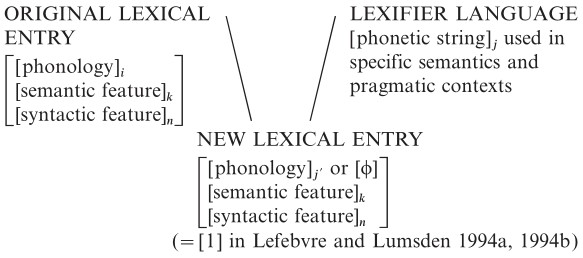
\includegraphics[scale=0.6]{general_model.jpg}
      \end{figure}

    \section{Haiti}
      Lefebvre uses the demographics of Haiti at the time when Haitian Creole was forming (i.e., 1680 to 1740) to delineate the possible source languages for different features that have appeared in the language.
      For European languages, she only writes about the presence of French, specifically the \lexi{langue d'oïl}, meaning the French spoken in northern and western France at that time.
      For African languages, the Atlantic, Mande, Kwa, Gur, Nigerian Benue-Congo, Ijoid, and Bantu language families were represented.
      Importantly, the speakers of these latter languages in Haiti were mostly adults.
      For this reason, Lefebvre posits that creole genesis is a process that primarily involves second language acquisition and therefore transfer of first language features.

    \section{Features}
      Lefebvre uses several features from Haitian Creole to illustrate how her model works.
      The first feature is one that she says was levelled almost immediately: third person plural pronouns and plural definite articles having the same phonetic form.
      In Fongbe, these two items do not in fact have the same phonetic form, yet they do in Ewe.
      However, Lefebvre knows of no attestations of a variety of Haitian Creole that has different forms for these two items, so she concludes that Fongbe speakers intially relexified their two lexical entries with different phonetic representations, but then quickly adapted to having only one form for both items to match the pattern of the Ewe speakers who only had one form for both right from the beginning.

      The second feature Lefebvre looks at is reflexive pronouns.
      In Fongbe, the reflexive pronoun is created using an affix that means something like \gloss{self} in the same way English does, whereas other African languages that were present use an affix that means either \gloss{head} or \gloss{body}.
      Since there is no good equivalent for a morpheme meaning \gloss{self} in French, the Fongbe speakers simply used a null morpheme, whereas the other speakers used either \lexi{tête} \gloss{head} or \lexi{corps} \gloss{body}, according to Lefebvre.
      The result is variation that persists to this day, showing that the levelling process does not have to occur quickly.

      Finally, Lefebvre discusses demonstratives as another example of a feature that has not levelled out.
      In this case, \lexi{sa} and \lexi{sila} exist in Haitian Creole today.
      For some speakers, one the former is only for proximal objects and the latter for distal objects, for others the former can also be distal at times, and still for others either one can be proximal or distal.
      Lefebvre argues that this is the case because the African languages spoken during the development of Haitian Creole differed in how they used demonstratives, and so these features were relexified differently and have persisted without being levelled over time.

    \section{Conclusion}
      Lefebvre argues that her model of relexification of different substrates, leading to variation, which is subsequently reduced through dialect levelling explains what one can find in Haitian Creole today.
      Her data is not vast, in this study at least, but does cover various circumstances.

    \printbibliography
\end{document}
